\section{Devices and Drivers}

Code reuse becomes difficult at the level at which algorithms 
communicate with the low-level hardware. The OS layer of YARP tries 
to minimize dependencies between algorithms and the hardware for 
which the operating system defines a constant interface (threading, 
memory, network, filesystem). Unfortunately more specific harware 
(motor control boards and framegrabbers are just 
popular examples) requires a more sophisticated mechanism. In these 
cases vendors provide device drivers and a set of API to simplify 
code development. The API comes in the form of a static or dynamic 
library which must be linked in the user code. Unfortunately
APIs vary a lot even within devices that belong to the same family. 
Even worse the API of the same hardware may vary on different 
operating systems or change on future releases. User code becomes 
dependent on the particular board for which it was initially developed 
and bound to the decisions and assumptions of the vendor. For 
example venodor A might decide to use integers to represent the position 
of a motor joint, wheras vendor B might decide to use a floating point
variable. More often even similar devices have different ``initialization'' 
procedure. Consider for example a motor control board which has a serial
interface to the host computer; the API of this board will probably require 
that some parameters (port number, baud rate, number of data bits, etc) are 
specified when the device is created. These parameters will be different 
those required by the API of the version of the board that has a USB 
interface (see \ref{fig:devices1}). When possible these (and other) 
differences must be hidden if we want that the same user code can 
effectively interface to the two devices.

\begin{figure}[tbp]
\centerline{
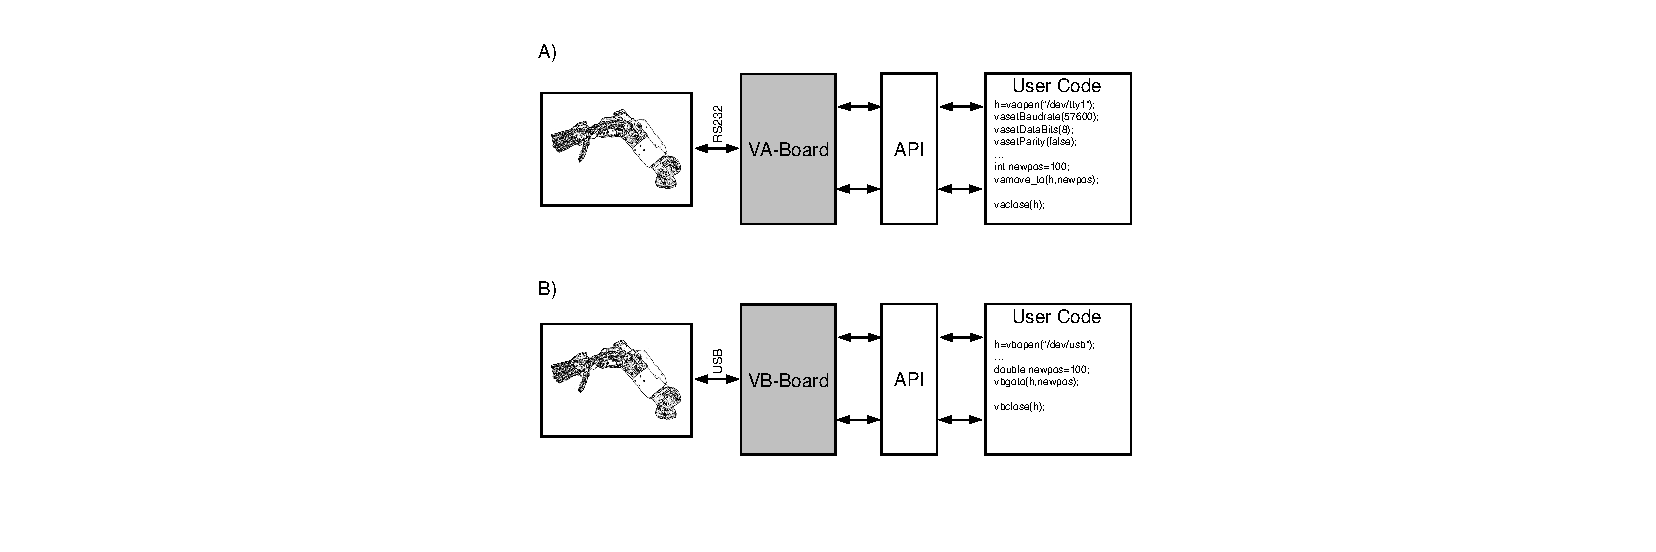
\includegraphics[width=24cm]{fig-devices1.eps}
}
\caption{Example of code dependency. VA-Board is a 
motor control board which interface to the robot through serial port. 
Changes in the board (in the example above the VB-Board uses USB) are 
propagated to the user code.}\label{fig:devices1}
\end{figure}

YARP implements the separation between user and device specific code 
in three ways: i) definition of interfaces for device families ii) 
separation of device initialization and creation from the rest of the code and 
ii) creation of network wrappers and separation between devices and 
communication. 

An interface to a YARP device is the specification of the functionalities
it provides. In practice in C++ an interface is a virtual base class, whose 
member functions define the ensamble of the functionalities a device must 
implement to be able to provide that interface. The implementation of a 
YARP device consists in a ``wrapper'' class which implements all 
methods specified by the interface. A single device can of course expose 
more than a single interface (in C++ this is implemented through multiple
inheritance). All details specific of the hardware 
(vendor's API and library) are handled here and are hidden by its interfaces. 
The idea is that changes in the hardware are catched by the wrapper class and never 
propagated to the user code. As a result, if interfaces are well designed,
 the impact on the code due to hardware change is minimized (see 
\ref{fig:devices2}). 

Interfaces to broad families of devices have been defined in YARP. Other families 
of devices defined in YARP are:

IFrameGrabberRgb, which defines the interface to devices which generate 
a stream of color images. Methods in this interface provide access to the most 
recent frame acquired by the device, and information about its size (number of 
columns and rows).

IFrameGrabberControls, specifies a set of functionalities to control a typical 
framegrabber device. Methods of this interface allows controlling the 
parameters of acquisition of the device, like shutter speed, brightness and gain.

Interfaces to motor control devices are more difficult to define. Control boards 
designed for industrial applications have often a quite stadard interface which 
provides a PID control algorithm and position or velocity control modes. Things 
become more complicated when we consider also programmable devices that can 
implement virtually an infinite type of functionalities and control algorithms. 
For this reason interface to control boards has been defined on the basis of 
the control paradigm they implement. Accordingly, YARP defines:

IEncoder: group all methods providing access to the motor encoders, like methods
for reading the current position of velocity of each axis

IPositionControl: methods to control motion of each axis by specifying its position
(usually referred to as ``position control'')

IVelocityControl: methods to contorl motion of each axis by specifying its velocity 
(usually referred to as ``velocity control'')

ITorqueControl: defiens methods to control the amount of force/torque exerted by 
each axis (usually referred to as ``torque or force control'').

These last three interfaces are indipendent of the particular algorithm the control
board implements to realize the corresponding functionality. These details are 
delegated to specific interfaces. For example IPidControl includes methods to 
interface to a PID controller, including methods to read or set the values of the 
gains.

All devices in YARP implements the DeviceDriver interface. The latter defines 
methods to manage the initialization and de-initialization of the device: 

\begin{verbatim}
  virtual bool open(yarp::os::Searchable& config)=0;
\end{verbatim}

This method opens the device. Parameters to the devices are passed to the
function as a list of key-value entries (a ``Searchable'' object). The latter 
can be specified in a text file (more details later).

\begin{verbatim}
virtual bool close()=0;
\end{verbatim}

This method performs all the operations required to close the 
device properly and release all the resources it was using. No
parameters are required by the function.

The DeviceDriver interface does not seem very useful at first. In practice this 
interface is never exposed to the user, and is used by a Factory object to create
the device. In YARP each device has a Factory object, which is responsible for 
creating the device and returning a pointer to it. This pointer is returned to 
the user and is the only ``access point'' to the device and its interfaces. Other 
interfaces can be objtained by casting this pointer to the appropriate virtual 
class (in C++ this can be safely done through dynamic cast). The PolyDriver object 
provides an interface to simplify the whole process of device creation, 
initialization and interface access.


\begin{figure}[tbp]
\centerline{
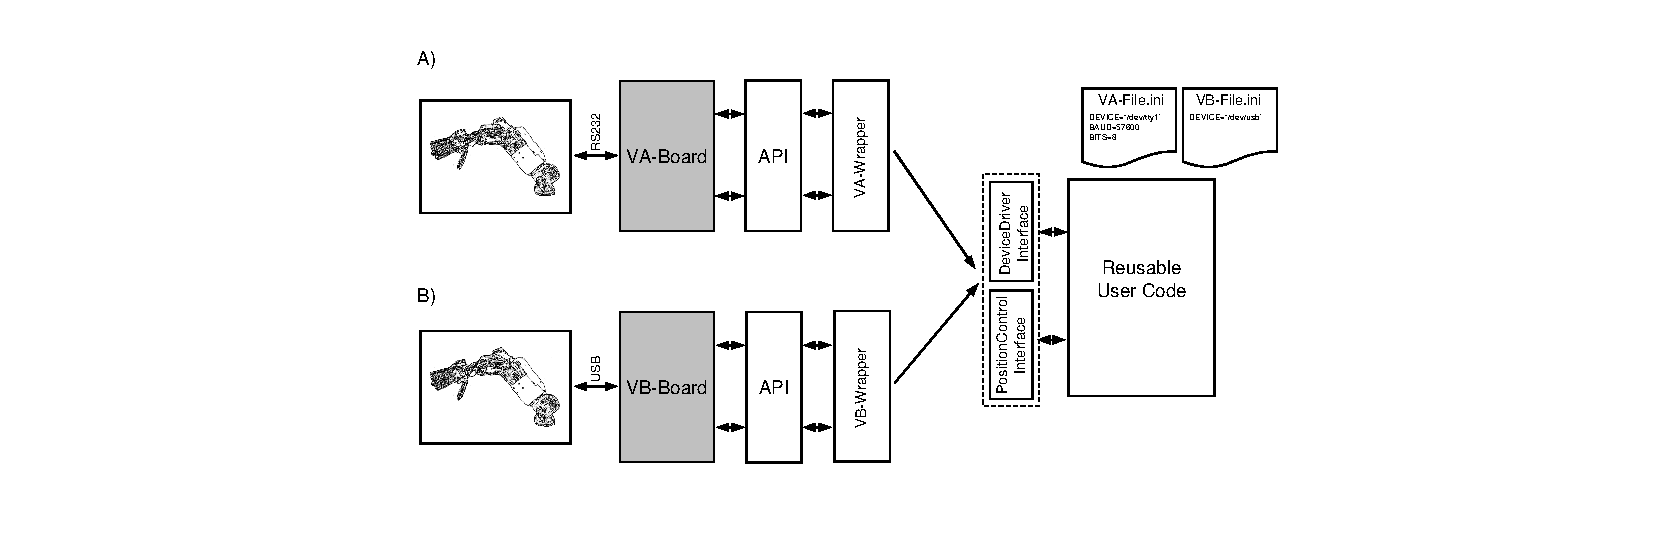
\includegraphics[width=24cm]{fig-devices2.eps}
}
\caption{Interfaces allow code reuse. VA-Board and VB-Boards now implemnt
the same interfaces (through their respective wrapper classes). The user 
code access the hardware through these interfaces and is not aware of 
the details of how the methods are actually implemented. The different 
initialization parameters are listed in configuration files and are thus 
separated from the code}\label{fig:devices2}
\end{figure}

\begin{itemize}

\item Summarize argument that, long term, free software approach 
is better for supporting devices especially with smaller user
bases, obsolescence.


\item Driver access in C/C++ with minimal bureaucracy -- no
entanglement with communication/middleware.  When operating
on a single machine, if the user wishes, operation without
transport or marshalling/demarshalling should be possible, ideally
direct C/C++ calls.

\item Ideally, drivers would be expressed in a form that
can be ``ripped out'' of any library or framework in use
with minimal hassle.

\item Similarly, a communication/middleware mechanism that is 
not tied up with the notion of drivers.

\item A communication/middleware mechanism that is transport
neutral, only depending on broad outline of services.


\end{itemize}




\subsection{Separation of concerns}

There are three separate concerns related to devices in YARP:

Implementing specific drivers for particular devices 

Defining interfaces for device families 

Implementing network wrappers for interfaces

Basic idea: if you view your devices through well thought out
interfaces, the impact of device change can be minimized.


\subsection{A light touch}

New devices come out all the time -- needs to be easy to connect them
to existing code

YARP needs a minimal ``wrapper'' class to match vendor-supplied
library with relevant interfaces that capture common capabilities

YARP encourages separating configuration from source code -- separating
the ``plumbing''

Devices and communications remain distinct concerns

(pictures)


\subsection*{Why?}

Allows collaboration between groups whose robots have different devices

Makes device changes less painful

Devices and communications are orthogonal features

Can switch from remote use of device to local use and vice versa without pain

Local use can be very efficient, just an extra virtual method call





\subsection{Sticky devices}

Consider the following scenarios:

\begin{itemize}

\item A user acquires a piece of hardware they want to use.  The
hardware is very new.  It is bundled with a binary library and a
skimpy example program that is the only way currently known to access
that hardware.  Use of the library is quite restricted; it may be
specific to a particular operating system version or even development
environment.

\item A user acquires many such devices, and wants to use them
all at the same time.

\end{itemize}

Let us call devices which can only be accessed using vendor supplied
material ``sticky devices'' because they tend to make the particular
set of assumptions made by the vendor stick to the user's code.
Dealing with several sticky devices at once becomes a nightmare.
Worse still, any and all of those assumptions could change on the
next release of the hardware~-- this is particularly likely if the 
hardware is very new.

A logical step in such a situation is to wrap the functionality
supplied by the vendor in a facade, so that at least source code
dependencies can be reduced.  But at a more basic level,
compilation and linking of application that accesses two or more
sticky devices can be very involved.  An option that YARP makes
available is for wrappers around the devices to be made individually,
compiled and built separately, and then used across the network.
When performance requirements permit this solution it is an
effective mechanism for quarantining the sticky devices.

We split the process of creating an interface to a device into two
parts: the ``thin wrapper'', and the ``network wrapper''.  

Writing the thin wrapper means creating a C++ API to the device
that follows a simple regular structure defined by YARP
(examples for interfacing with devices are usually written in C/C++).
If there are similarities between this device and others,
those similarities can be captures at this point by 
shared interfaces with different implementations.
Once the thin wrapper is written, user code that accesses
the device through that wrapper is less affected by its ``stickiness''
because:

\begin{itemize}

\item To the extent that user code uses interfaces shared by other
devices, another device can be substituted later without change to
that part.  This could also include future versions of the same family
of hardware.

\item The network wrapper, when written, will allow the thin wrapper
interface to be used via the network.  This decouples the compilation,
build environment, libraries, operating system, and language
dependencies of the device software and the user software.

\end{itemize}

Wrappers are written for families of interfaces, and so in as much
as one device is similar to existing devices, the network 
wrapper may come for free.

Why is it important to make devices easy to write?

\begin{itemize}

\item New hardware appears all the time, so the odds of a particular
user being one of the first people interested in a particular device are
non-negligible.  We are particularly interested in supporting humanoid
robotics, where today's hardware is very lacking and we are guaranteed
to be dealing with novel hardware for the forseeable future.

\item Vendors may bundle hardware and software, and not permit
redistribution of their software.  In practice, this can mean that
work done to wrap a device by one group may not end up in a public
repository, and so not reach other groups.  Licensing issues can push
the amount of effort required above what a group is willing to
casually contribute.  So some reinventing of the wheel is inevitable.
This seems to be particularly the case on the Microsoft Windows
platform, where the pool of free and open software available to build
on is smaller and much more poorly packaged.

\item There are several software architectures in existence for
various overlapping robotics communities.  If someone has adapted
a device to one of these architectures, it is still not trivial
to use it in another.  YARP is trying to be a good citizen by
reducing how much the core device code depends on YARP itself,
making it in principle easier to reuse.


\end{itemize}



\subsection{The many-architecture problem}

YARP is but one software architecture of many.  For example, in the
world of mobile robotics, the Player/Stage project is widely used.

We should be careful of assuming that the interface the end-user will
want to the device is a YARP interface.

The thin wrapper is a first step that attempts to reshape a
device from a vendor into something a little bit more organized.

The trajectory imagined for device creation:

\begin{itemize}

\item User works with whatever code they can get -- vendor
supplied, from another project, etc.

\item User wraps a simple class around the functionality,
meeting YARP's simple specification for devices.  At this
point, the reward they get is that device configuration
can be easily made external to the code.  This is often
useful when starting up a device for different purposes
(normal, testing, different experimental parameters etc).

\end{itemize}


\subsection{Driver}

We use the term ``Driver'' to refer to software interface the end-user
has to a hardware device.  The software components involved in
implementing the driver can be considered to be part of the device if
we wish.  We can consider the process of taking a ``sticky device''
and placing in a wrapper as a process of transforming the device such
that drivers are easier to build.


